\chapter{Antecedentes}
\label{sec-2}

\label{cap:antecedentes}

  Para poder describir correctamente tanto el problema como la
  solución implementada, es necesario dar los punteros y conceptos
  básicos que los involucran. En este capítulo se discutirán los
  siguientes tópicos:

\begin{itemize}
\item La red social Twitter, la cual es utilizada como fuente de datos y
    documentos para este trabajo.
\item Clustering de documentos, y en general, estrategias de clustering,
    las cuales tienen muchas aplicaciones prácticas. En este trabajo
    fue utilizada una de estas estrategias para poder determinar los
    subtópicos de cada evento.
\item La identificación automática de eventos, la cual, si bien se
    utilizó un enfoque más simple para este trabajo, sirve para
    indicar en qué aspectos es posible extender este trabajo en el
    futuro.
\item Resúmenes automáticos: una sucinta definición, y algunos enfoques
    que han existido en el tiempo para este procedimiento.
\item Ranking de documentos, o cómo generar órdenes de acuerdo a
    relevancia.
\end{itemize}
  Casi todos estos tópicos, a excepción del primero, involucran
  técnicas de Minería de Datos, Recuperación de la Información y
  Aprendizaje de Máquinas, entre otras áreas.

\section{Twitter}
\label{sec-2.1}

   Twitter es una red social online que permite conectar a
   personas mediante la comunicación de mensajes cortos, rápidos y   frecuentes\footnote{\href{https://support.twitter.com/groups/31-twitter-basics/topics/104-welcome-to-twitter-support/articles/13920-get-to-know-twitter-new-user-faq}{https://support.twitter.com/groups/31-twitter-basics/topics/104-welcome-to-twitter-support/articles/13920-get-to-know-twitter-new-user-faq} }. Estos
   mensajes son publicados en el perfil del usuario que los emite,
   pueden ser vistos directamente por los seguidores de este usuario o
   ser vistos directamente en el perfil o buscándolos mediante una
   funcionalidad que provee el servicio. Además, un usuario puede
   \emph{seguir} a otros para poder ver en su \emph{timeline} o perfil privado
   los mensajes de todos a quienes sigue.

\begin{figure}[h!b]
  \centering
  
\includegraphics[width=12cm]{./img/twitter.png}
  \caption[Timeline de Twitter.]
   {Timeline de Twitter. En éste se ve una lista en orden cronológico
  de los tweets generados por los usuarios que sigue el usuario
  actual. Además, el sitio incluye tweets promocionados por cuentas
  que pagan por dicho servicio, como es el caso del primer tweet en la
  lista.}
\end{figure}

   Estos mensajes, o \emph{tweets}, sólo son cadenas de caracteres con
   metadatos que el mismo servicio asigna una vez enviado a la red
   social. Desde sus inicios (año 2007) se han añadido algunas capacidades
   adicionales a estos mensajes, como la de poner URLs, imágenes,
   vídeos, etc. Además, existen varias convenciones que han surgido a
   lo largo del tiempo. A continuación se describe una lista de tipos
   de mensajes que existen en Twitter, originados por estas convenciones:

\begin{enumerate}
\item Respuestas o \emph{replies}: son mensajes del tipo \texttt{@usuario [texto]},
      que ocurren usualmente en una conversación entre dos usuarios.
\item Menciones o \emph{mentions}: un poco más general a una respuesta, el
      nombre del usuario mencionado puede estar en cualquier parte del
      mensaje. La diferencia semántica es que no se le habla
      ``directamente'' al usuario mencionado, como en una respuesta, sino
      que sólo es mencionado por si el mensaje es de su interés o no.
\item \emph{Retweets}: son mensajes del tipo \texttt{RT @usuario: [texto]}. Ocurren
      cuando se quiere compartir el mensaje de otro usuario, o citarlo
      para mencionarlo en el mismo mensaje.
\item \emph{Hashtags}: son palabras precedidas por el caracter \#, que indican
      un identificador a cierto evento o suceso dentro o fuera de la
      red. Suelen usarse para categorizar de cierta forma un tópico, pero
      son libres de usarse como los usuarios quieran.
\item Mensaje simple: un mensaje sin menciones ni hashtags.
\end{enumerate}
  Ejemplos:

\begin{itemize}
\item Mensaje simple: \texttt{Jason Funk disipa patitos};
\item Respuesta: \texttt{@jason estoy de acuerdo con lo que dices};
\item Mención: \texttt{creo que @jason es una cumbre de sabiduría};
\item Retweet: \texttt{RT @jason: Jason Funk disipa patitos}; y
\item Hashtag: \texttt{Estoy escribiendo mi memoria \#dcc \#summarization}
\end{itemize}
  Estos mensajes están limitados a 140 caracteres de extensión. Sumando
  esto a la integración de la red con otros servicios y dispositivos, y
  a la cantidad de mensajes publicados cada minuto, permite utilizar
  esta red como una gran fuente de datos.

  Twitter además provee varios servicios adicionales, como por ejemplo,
  un servicio de acortamiento de URLs, para permitir incluir una URL
  larga sin perjudicar la cantidad de caracteres restantes para el
  mensaje; un servicio de alojamiento de fotos y vídeos, para hacer más
  sencilla la publicación de mensajes multimedia desde dispositivos
  móviles; un servicio de búsqueda que permite buscar una cantidad
  determinada de tweets sobre un término de búsqueda o un hashtag,
  entre otros servicios.







\section{Clustering de documentos}
\label{sec-2.2}


   El análisis de clusters o clustering es el proceso de encontrar
   grupos de objetos, tal que los objetos en un grupo sean similares
   entre sí (o relacionados) y que sean diferentes (o no relacionados)
   a los objetos de otros grupos. Algunas aplicaciones del análisis de
   clusters son, entre otras:
\begin{itemize}
\item Encontrar clusters naturales y describir sus propiedades (\emph{data understanding});
\item Encontrar agrupamientos útiles (\emph{data class identification});
\item Encontrar representantes de grupos homogéneos (\emph{data reduction});
\item Encontrar perturbaciones aleatorias de los datos (\emph{noise detection});
\item Encontrar objetos inusuales (\emph{outliers detection});
\item etc.
\end{itemize}
   Se denomina cluster a un grupo de objetos, mientras que
   clustering puede referirse al conjunto de clusters o al proceso de
   encontrarlos. Existen diversos tipos de procesos de clustering, una
   de las distinciones más importantes es entre los clusters
   jerárquicos y los particionales:
\begin{itemize}
\item Un clustering jerárquico es un conjunto de clusters anidados,
     organizados más bien como un árbol. Cortando el árbol en
     cualquier nivel da como resultado un clustering potencialmente
     distinto.
\item El clustering particional es un conjunto de clusters de forma de
     partición del conjunto total, es decir, cada objeto está
     contenido en un sólo subconjunto o cluster.
\end{itemize}
   Para describir el proceso aplicado a documentos, primero se
   describirán los modelos de representación más importantes para,
   de forma de definir la noción de documento y luego los
   algoritmos de clustering aplicados a éstos.

\subsection{Modelos de representación de documentos}
\label{sec-2.2.1}


    \subsubsection{Standard Boolean Model}

    El modelo booleano es un modelo de representación de
    documentos. En él, los documentos son vectores de \emph{términos}:

    $$d = (w_1,w_2,\ldots,w_m)$$

    Donde un término es un $n$-grama del texto del documento.

    \begin{defn} Un $n$-grama es una secuencia contigua de $n$ ítems a
    partir de un texto. \end{defn}

    La definición de ítem dependerá de la aplicación: en lenguaje
    natural el texto a su vez dependerá del idioma, por ejemplo, si el
    texto está en inglés o en japonés, la distinción entre palabras
    es distinta para cada uno.

    No existe una medida de ``similitud'' como tal en este modelo, sino
    que se considera el calce exacto entre los términos de una query
    $q$ y un documento $d$. La query puede ser una consulta hecha por
    un usuario al conjunto de documentos, o bien un documento del
    mismo conjunto.

    Una consulta es una fórmula de lógica proposicional que pide los
    documentos que contengan o no ciertos términos.

    \subsubsection{Bag of words Model}

    En el modelo Bag of Words un documento $d$ es representado como un
    conjunto de pares $(w_i, f_i)$, $i\in[1..m']$, donde $w_i$ es un
    término del documento, $f_i$ es la frecuencia de $w_i$ en el
    mismo, y $m'$ es la cantidad de términos distintos en el
    documento.

    La ventaja principal por sobre el modelo anterior es que permite
    hacer calces parciales entre consultas y documentos. Este modelo
    es comúnmente utilizado para hacer clasificación de documentos,
    por ejemplo, para determinar si un correo electrónico es o no
    spam.

    \subsubsection{Vector Space Model}

    El \emph{Vector Space Model} es un modelo un poco más general que el
    anterior. Un documento $d$ es representado como un vector de pesos
    asociados a los términos:

    $$d = (f(w_1), f(w_2), \ldots, f(w_m))$$

    Cada dimensión de este vector corresponde al peso asociado a un
    término del documento.

    El peso puede ser directamente la frecuencia del término dentro
    del documento:

    $$\freq(w,d) = |\{w : w \in d\}|$$

    O bien, normalizar esta frecuencia para evitar que documentos más
    largos sean más relevantes sólo por su extensión:

    $$\tf_0(w,d) = \left\{
    \begin{array}{l l}
    1 & \quad \textrm{si $w \in d$}\\
    0 & \quad \textrm{si no}\\
    \end{array} \right.$$

    $\tf_0$ o \emph{Term Frequency} es una primera aproximación a medir la
    frecuencia de un término en un documento. Sin embargo, esta nueva
    aproximación sufre de la desventaja de que ahora un documento con
    una ocurrencia del término será igual de relevante que algún
    documento que mencione varias veces el término (por ejemplo, un
    diccionario que tiene el término una vez contra un artículo sobre
    el tema). Otra alternativa, considera no castigar demasiado a los
    documentos con pocas ocurrencias, pero tampoco beneficiar mucho a
    los que tengan muchas:

    $$\tf_1(w,d) = 1 + \log(\freq(w,d))$$

    La solución más utilizada considera la proporción con respecto al
    término con más ocurrencias, para esto, se normaliza por el tamaño
    del documento:

    $$\tf(w,d) = \frac{\freq(w,d)}{max\{\freq(t,d) : t \in d\}}$$

    Otro problema que tiene utilizar esta medida como los pesos de los
    términos, es que un término muy repetido entre todos los
    documentos que hablan de un mismo tema puede significar que no es
    muy relevante (por ejemplo, las \emph{stopwords} o palabras vacías, son
    por lo general las preposiciones, artículos, pronombres,
    etc.). Para esto, se considera además ponderar por el inverso de
    la frecuencia entre los documentos; es decir, un término frecuente
    entre todos los documentos ve su peso castigado a diferencia de un
    término que sólo es mencionado una vez en un documento. Esta
    medida es llamada \emph{Inverse Document Frequency} o $\idf$:

    $$\idf(t, D) = \log \frac{ |D| } {1 + |\{d \in D : t \in d\}| }$$

    Finalmente, el peso de un término es la ponderación de su
    frecuencia dentro del documento con el inverso de la frecuencia
    entre los documentos, o $\tfidf$:

    $$\tfidf(t,d,D) = \tf(t,d) \times \idf(t,D)$$

    Para el resto de este trabajo se considerará la representación de
    documentos en este modelo.

\subsection{Medidas de similitud}
\label{sec-2.2.2}


    A lo largo de los años, dos formas han sido las usuales para
    determinar similitud entre
    documentos\cite{Zhao02criterionfunctions}: calculando el coseno de
    los dos vectores, y la distancia euclidiana.

    El coseno de dos documentos $d_i$ y $d_j$ se define como

    $$\cos(d_i, d_j) = \frac{d_i^td_j}{\|d_i\|\|d_j\|}$$

    Si ambos $d_i$ y $d_j$ son iguales, entonces la fórmula anterior
    se evalúa a 1, y 0 si no tienen nada en común, es decir, ambos
    vectores son ortogonales.

    La distancia euclidiana entre $d_i$ y $d_j$ se define como

    $$d(d_i,d_j) = \sqrt{(d_i-d_j)^t(d_i-d_j)} = \|d_i-d_j\|$$

    En este caso, si la distancia es 0, entonces ambos documentos son
    idénticos. Y si ambos son ortogonales, la distancia será
    $\sqrt{2}$.

    Si ambos documentos están normalizados (su norma es 1), entonces
    ambas medidas serán muy parecidas, aun así siendo una de similitud
    y la otra de distancia.

\subsection{Algoritmos de clustering}
\label{sec-2.2.3}


    Se considerará la siguiente definición para el problema de
    clustering:

    Dado un entero $k$ y un conjunto de $n$ puntos en $\mathbb{R}^v$,
    el objetivo es determinar $k$ puntos tal que se minimice $\phi$,
    la suma de las distancias al cuadrado de cada punto y su centro
    más cercano.

    Este problema es NP-hard, sin embargo, existe un algoritmo que
    permite realizar una búsqueda local y determinar $k$ centros
    en un tiempo razonable.

    K-means\cite{Lloyd:2006:LSQ:2263356.2269955} es un algoritmo de
    clustering particional, en el cual cada cluster tiene un
    \emph{centroide} asociado, esto es, típicamente, un punto
    el cual es el promedio de todos los puntos del cluster, y no
    necesariamente corresponde a un dato real.

    El algoritmo genera $k$ clusters, donde $k$ es un parámetro del
    algoritmo, tal que cada punto pertence al cluster cuyo centroide es el
    más cercano a éste.

\begin{algorithm}[H]
 \KwData{$k>0$, conjunto $D$ de puntos}
 \KwResult{Asignación de cada punto a un cluster $i \in [1..k]$}
 Seleccionar $k$ puntos como centroides iniciales\;
 \While{Los centroides cambien a cada iteración}{
  Formar $k$ clusters asignando todos los puntos al centroide más cercano\;
  Recalcular los centroides de cada cluster\;
 }
 \caption{K-means}
\end{algorithm}

    Los clusters generados dependerán de la elección inicial de los
    centroides, y usualmente basta con pocas iteraciones para la
    convergencia. La complejidad de este algoritmo es $O(nkIv)$, donde $n$
    es el número de puntos, $k$ el parámetro de la cantidad de clusters,
    $I$ es la cantidad de iteraciones que hará el algoritmo y $v$ es la
    cantidad de dimensiones de los vectores.

    K-means también puede verse desde el enfoque de optimizar una
    función criterio. La medida más común es la
    \emph{suma del error cuadrado} o Sum of Squared Error (SSE). Para cada
    punto, su \emph{error} es la distancia al cluster más cercano:

    $$SSE = \sum_{i=1}^k\sum_{x\in C_i} \dist^2(m_i,x)$$

    Donde $x$ es un punto en el cluster $C_i$, y $m_i$ es su
    centroide. La distancia $\dist$ suele ser distancia euclidiana
    entre los dos puntos. Dados dos clusters, en cada paso se escoge
    el que tenga menor error.

    K-means converge rápidamente a un óptimo, sin embargo, éste puede
    ser un óptimo local, dado que es altamente dependiente de la
    elección de los centroides iniciales. Dado que la probabilidad de
    acertar a los centroides
    ``reales'' (precisión) es muy baja, es posible que un clustering
    tenga un mal error cuadrático, de hecho, el radio competitivo con
    la solución óptima es no acotado incluso para $k$ y $n$ fijos.
    Existen varias formas de evitar
    este problema, por ejemplo, ejecutando varias veces K-means,
    usar clustering jerárquico para determinar los centroides
    iniciales, determinar más de $k$ centroides y luego elegir los $k$
    más separados, etc.

    Un enfoque utilizado es el de usar el algoritmo
    K-means++\cite{Arthur:2007:KAC:1283383.1283494}, el cual tiene
    como objetivo determinar los centroides iniciales para
    K-Means. Este algoritmo garantiza un radio competitivo de
    $O(\log k)$ con respecto al error cuadrático esperado del óptimo.
    El algoritmo K-means++ escoge los centroides con cierta
    probabilidad que depende de la distancia al centroide más cercano,
    lo cual garantiza una buena elección inicial, y luego continúa con
    el algoritmo usual. Sea $D(x)$ la distancia de $x$ al centroide
    más cercano. El algoritmo es como sigue:

\begin{algorithm}[H]
 \KwData{$k>0$, conjunto $D$ de puntos}
 \KwResult{Asignación de cada punto a un cluster $i \in [1..k]$}
Escoger un centroide $c_1$ al azar uniformemente de $D$\;
Escoger un nuevo centroide $c_i$, escogiendo $x \in D$ con probabilidad $\frac{D(x)^2}{\sum_{x' \in D}D(x')^2}$\;
Repetir paso 1 hasta haber escogido $k$ centros\;
Proceder con K-means estándar\;
 \caption{K-means++}
\end{algorithm}


    Existen muchas otras variantes para resolver el problema de
    clustering, principalmente dependientes de la naturaleza de los
    datos. En la Figura\footnote{Imagen obtenida de \href{http://scikit-learn.org/dev/auto\_examples/cluster/plot\_cluster\_comparison.html}{http://scikit-learn.org/dev/auto\_examples/cluster/plot\_cluster\_comparison.html} }
     \ref{fig:clusters} se puede apreciar una
    comparación entre distintos algoritmos de clustering y los
    resultados obtenidos. MiniBatch K-means es una variante de K-means
    que mejora sustancialmente el tiempo de convergencia escogiendo
    subconjuntos en vez de centroides al inicio, aunque la calidad de
    los resultados puede ser levemente menor a la del algoritmo
    clásico\cite{Sculley:2010:WKC:1772690.1772862}.

\begin{figure}[h!b]
  \centering
  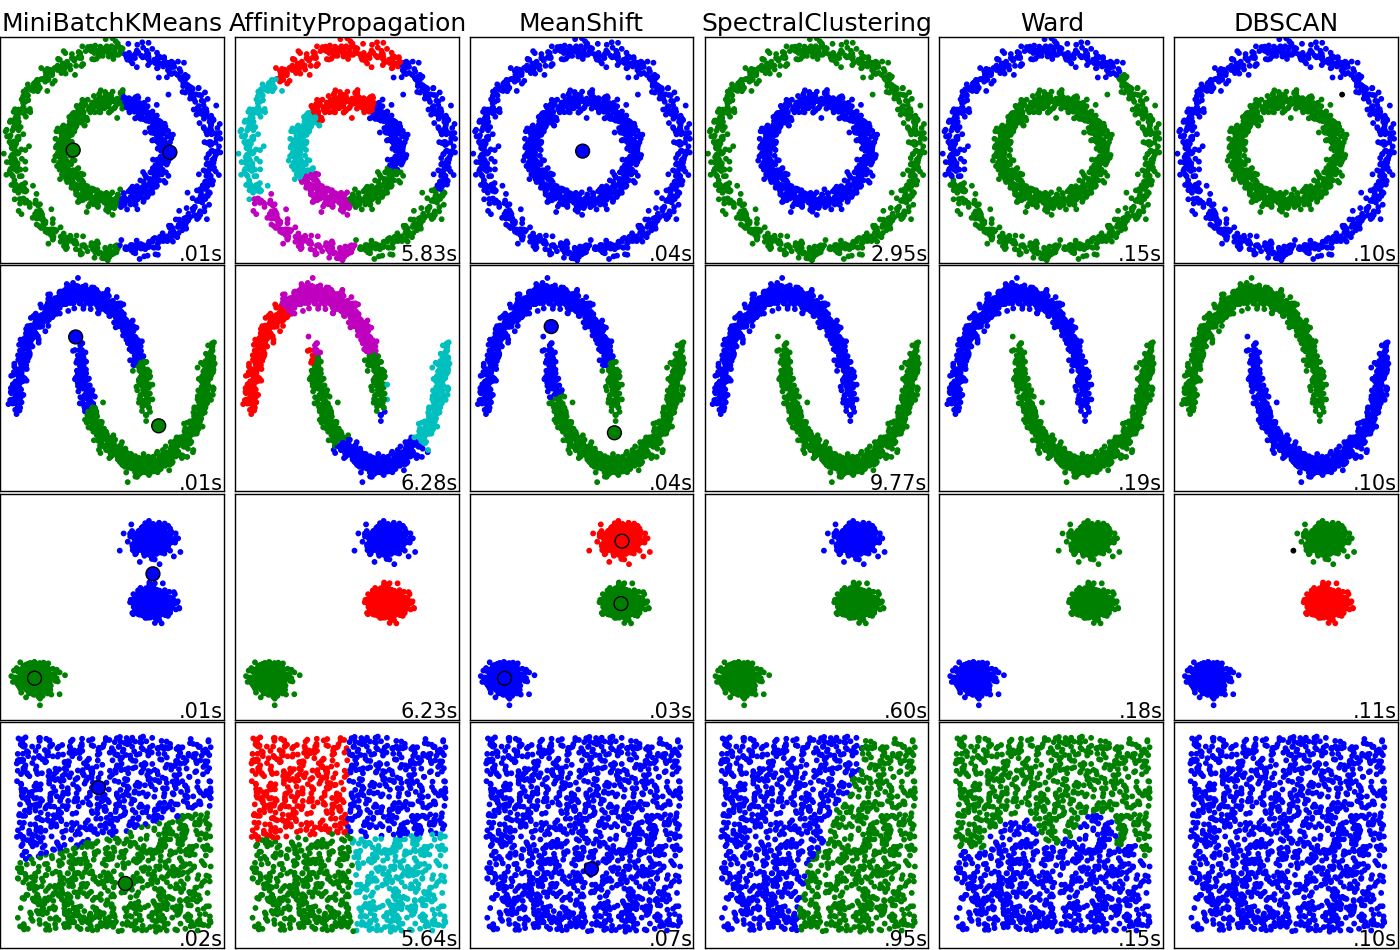
\includegraphics[width=16cm]{./img/cluster_comparison.png}
  \caption[Comparación de algoritmos de clustering]
   {Comparación de algoritmos de clustering\label{fig:clusters}. En la
  figura se muestran las características de distintos algoritmos de
  clustering sobre datos en 2 dimensiones. El último caso muestra
  datos uniformes en el cual sólo habría 1 cluster.}
  \end{figure}

\subsection{Evaluación de clusters}
\label{sec-2.2.4}


    Existen dos enfoques para evaluar clusterings: validación interna
    y externa\footnote{\href{http://en.wikipedia.org/wiki/Cluster\_analysis\#Evaluation\_of\_clustering\_results}{http://en.wikipedia.org/wiki/Cluster\_analysis\#Evaluation\_of\_clustering\_results} } La validación interna considera evaluar el clustering
    con respecto a los datos que han sido agrupados (es decir, sin
    información adicional), mientras que la evaluación externa
    considera datos adicionales, como etiquetas a los datos
    determinadas con anterioridad.

    La idea básica detrás de las medidas internas directamente de la
    definición de clustering. Una buena solución debería agrupar
    objetos en varios clusters, de forma que los objetos dentro de un
    cluster sean más similares entre sí, y que los objetos de clusters
    distintos lo sean lo menos posible. La calidad de la solución se
    mide en términos del promedio de la similitud interna, y en
    términos del promedio de la similitud externa, y el radio entre
    estos dos promedios. Entre más alto es el radio, mejor es la
    solución entregada.

    Por otra parte, dos de las métricas para validación externa más
    usadas para evaluar clusterings, segun
    \cite{Zhao02criterionfunctions} son:

\begin{itemize}
\item \textbf{Entropía}: mide cómo son distribuidas las clases de documentos
      entre cada cluster. Se define formalmente como

      $$E(C_r) = -\frac{1}{\log q}\sum_{i=1}^q\frac{n^i_r}{n_r}\log\frac{n^i_r}{n_r}$$

      donde $q$ es el número de clases en el dataset, y $n^i_r$ es el
      número de documentos de la $i$-ésima clase que fue asignado al
      $r$-ésimo cluster $C_r$. La entropía del clustering se define
      como la suma ponderada de la entropía de cada cluster:

      $$\textrm{Entropia} = \sum_{r=1}^k \frac{n_r}{n} E(C_r)$$

      Un clustering perfecto tendrá clusters tal que cada cluster
      contenga documentos de una sola clase, en ese caso la entropía
      será 0. En general, conviene tener bajos valores de entropía.
\item \textbf{Pureza}: mide la cantidad de documentos de la clase más grande
      en un cluster dividida por el tamaño del cluster. La pureza de
      un cluster $C_r$ se define como

      $$P(C_r) = \frac{1}{n_r} \Mmax_i\{n^i_r\}$$

      A mejor pureza, mejor es la solución.
\end{itemize}
\section{Identificación automática de eventos}
\label{sec-2.3}


   La identificación automática de eventos consiste en, dado un
   conjunto de documentos, donde cada documento está asociado a un
   evento (desconocido), poder particionar el conjunto de
   documentos en clusters, de forma que cada cluster corresponda a
   todos los documentos asociados a un evento.

   La definición de ``evento'' dada por
   \cite{Yang:1999:LAD:630307.630471}, considera lo siguiente:

   \begin{defn} Un \emph{evento} es un suceso que ocurre en un período de tiempo
   determinado y en un lugar específico. \end{defn}

   Otra definición de ``evento'' considera además la información
   asociada a éste\cite{allan2002topic}:

   \begin{defn} Un \emph{evento} es una ocurrencia en el mundo real $e$ con
   (1) un período de tiempo asociado $T_e$, y (2) una secuencia
   ordenada cronológicamente de mensajes $M_e$ de volumen sustancial,
   que discuten la ocurrencia y que son publicados durante el período
   $T_e$ \end{defn}

   Si los eventos son conocidos con anticipación, el problema consiste
   en recuperar documentos que los discutan. Las fuentes de datos son
   por lo general muy especializadas, por ejemplo, en el caso de las
   noticias\cite{Diakopoulos:2012:FAS:2208276.2208409} o documentos
   estructurados, donde es posible utilizar técnicas de procesamiento
   de lenguaje natural para detectar características de los documentos
   y utilizar un clasificador para identificar el evento al cual
   pertenecen. Algunos trabajos utilizan otras fuentes de datos, tal
   como de fotografías o vídeos, donde estas tienen sus propias
   características (descripción, tags, coordenadas geográficas,
   marca de tiempo, etc.), las cuales son aprovechadas para
   aplicaciones ad-hoc\cite{Liu:2011:USM:2072609.2072613}. Otros
   esfuerzos consideran utilizar distintas fuentes de datos y aprender
   sus características, combinándolas todas utilizando alguna
   metodología entrenada con anticipación, tales como
   \cite{Becker:2010:LSM:1718487.1718524}, o
   \cite{Becker:2012:ICP:2124295.2124360}, en el cual se generan
   distintas queries de manera automática para realizar búsquedas de
   documentos en la Web, basadas en las características de los
   eventos. Esto permite  enriquecer los  eventos con información
   variada sobre ellos.

   Cuando los eventos no son conocidos con anticipación, algunos de
   los enfoques mencionados anteriormente también pueden ser
   utilizados, por ejemplo, suponer que ocurre un evento si muchos
   documentos (imágenes, vídeos, tweets, etc.) fueron generados en la
   misma zona geográfica en un período acotado de tiempo, como en
   \cite{Liu:2011:USM:2072609.2072613}, o si se publican muchos
   mensajes de un tópico en particular en un período acotado (llamado
   un \emph{burst} o ráfaga de mensajes); en ese caso también se pueden
   identificar eventos cuando el tópico es conocido, por ejemplo, en
   \cite{chakrabarti2011event} utilizan eventos deportivos para
   identificar las partes más relevantes de cada partido, basándose en
   los bursts de tweets ocurridos en Twitter.


\section{Resúmenes automáticos}
\label{sec-2.4}


   Debido a la gran cantidad de información en Internet, los sistemas
   de \emph{Information Retrieval} (IR) se volvieron necesarios para la
   extracción de contenido relevante a partir de los documentos
   encontrados. Sin embargo, dada aún la gran cantidad de documentos
   retornados por estos sistemas, un siguiente nivel de abstracción ha
   sido necesario para éstos, el cual es la necesidad de construir
   resúmenes de estos documentos\cite{Ganapathiraju_relevanceof}. Un
   survey más exhaustivo sobre el tema puede ser consultado en
   \cite{Das07asurvey}.

   Entre las múltiples aplicaciones de los resúmenes automáticos se
   pueden mencionar:
\begin{itemize}
\item Extracción de información de múltiples fuentes;
\item Rápida adquisición de conocimiento;
\item Responder preguntas automáticamente de tópicos muy específicos;
\item Generación de reseñas biográficas, etc.
\end{itemize}
   Los resúmenes pueden ser clasificados según los siguientes
   criterios:

\begin{itemize}
\item \textbf{Detalle}: Indicativo / Informativo;
\item \textbf{Granularidad}: Específico a un evento / Mirada general;
\item \textbf{Técnica}: Extractivo / Abstractivo;
\item \textbf{Contenido}: Generalizado / Basado en consulta; y
\item \textbf{Aproximación}: Dominio / Específico de un género /
     Independiente.
\end{itemize}
   Las categorías más importantes a la hora de clasificar un resumen
   son la técnica y el contenido, mientras que otra forma de
   clasificar resúmenes se basa en la entrada de la aplicación:
   resumen de un solo documento o bien multi-documento.

   Un resumen extractivo apunta a
   extraer las oraciones más importantes de un documento, mientras
   apunta a mantener una baja redundancia en el resumen. Un resumen
   abstractivo es más complejo: la idea es poder generar un resumen
   utilizando palabras no necesariamente sacadas de los documentos, o
   dicho de otra forma, estos sistemas intentan \emph{comprender} el
   contenido de los documentos de forma de generar un resumen
   abstracto. La forma clásica de generar resúmenes es utilizando
   métodos extractivos, dada la complejidad y baja calidad aún de los
   enfoques abstractivos.

   El criterio de contenido de un resumen se basa principalmente en
   cuál es la base para generarlo: si es basado en consulta, entonces
   la entrada del sistema es una frase y el resumen intenta encontrar
   las frases u oraciones más similares a la consulta, como una
   especie de respuesta a una pregunta. Un resumen de contenido
   general simplemente genera un resumen de todo el o los documentos
   de la entrada.

   Existen diversos enfoques para generar un resumen en base a uno o
   múltiples documentos: el más usual es utilizando clustering. Sin
   embargo, a veces son consideradas algunas características propias
   del documento: por ejemplo, si son noticias, usualmente las
   primeras oraciones del texto contienen la información más
   relevante\cite{DBLP:conf:spire:Bravo-MarquezM12}. Algunas
   características generales usuales son:

\begin{itemize}
\item Ocurrencia de palabras clave: oraciones con palabras
     clave usualmente son usadas en el resumen.
\item Palabras claves de título: a su vez, oraciones que contengan
     palabras del título también son consideradas importantes.
\item Heurísticas de ubicación: como fue mencionado, según la
     naturaleza del documento, la ubicación de las frases tienen
     cierta relevancia, tales como en documentos noticiosos, o
     artículos técnicos.
\item Frases indicativas: ``en este informe'', o ``en conclusión''.
\item Frases cortas: usualmente las frases muy cortas no son tomadas en
     consideración.
\item Características de palabras en mayúsculas: acrónimos o nombres
     propios son considerados importantes.
\end{itemize}
   Entre las distinas estrategias para generar resúmenes, aparte de
   clustering usando una representación adecuada de los documentos, se
   cuentan:

\begin{itemize}
\item Similitud directa entre documentos, usando el coseno de los
     vectores;
\item Aproximaciones usando teoría de grafos, en el cual, por ejemplo,
     cada nodo es una frase, y una arista existe entre dos nodos si su
     similitud está sobre un umbral; luego se determina la centralidad
     de los nodos mediante un camino aleatorio u otras estrategias;
\item Usando aprendizaje de máquinas: mediante un clasificador aprender
     las características de un conjunto de prueba;
\item Utilizando modelos más elaborados, como Modelos Ocultos de
     Markov\footnote{\href{http://en.wikipedia.org/wiki/Hidden\_Markov\_model}{http://en.wikipedia.org/wiki/Hidden\_Markov\_model} }
     para determinar características ocultas entre los datos, como fue
     usado en \cite{chakrabarti2011event}; etc.
\end{itemize}
\subsection{Evaluación de resúmenes}
\label{sec-2.4.1}


    ROUGE (\emph{Recall Oriented Understudy for Gisting Evaluation})\cite{Lin:2003:AES:1073445.1073465}
    es una medida intrínseca para la evaluación semi-automática de
    resúmenes. No es tan efectiva como una evaluación hecha por
    humanos, dada la naturaleza del problema, pero es más conveniente
    y escalable.

    Dado un documento $D$ y su resumen automático $X$, y $M$ personas
    que generan un resumen de referencia sobre $D$, ROUGE-$n$ se
    determina de la siguiente forma:

    $$\rouge\text{-}n = \frac{  \sum_{S \in \MREF} \sum_{\ngram i \in S} \Mmin( \Mcount(i,X),\Mcount(i,S) )   }{ \sum_{S\in \MREF}\sum_{\ngram i \in S}  \Mcount(i,S) }$$

    Donde $\MREF$ es el conjunto de resúmenes de referencia, y
    $\Mcount$ cuenta las ocurrencias del $n$-grama $i$ en $X$ o
    $S$. $\rouge\text{-}n$ mide la cantidad de $n$-gramas de los
    resúmenes de referencia que aparecen en el resumen automático, por
    lo que es necesario que hayan muchos resúmenes de referencia dada
    la potencial subjetividad a la que son sujetos.

\section{Ranking de documentos sociales}
\label{sec-2.5}


   Siguiendo este proceso, primero identificando eventos, luego
   generando resúmenes a partir de ellos, el último paso corresponde a
   determinar, a partir de un conjunto pequeño de documentos (que si
   bien, no corresponden directamente a un \emph{resumen} de acuerdo a lo
   dicho en la sección anterior, puesto que estos resúmenes consideran
   la extracción de frases a partir de los documentos, y no documentos
   enteros), cómo determinar cuáles son más relevantes que otros. Otra
   aplicación directa consiste en determinar, más que relevancia,
   \emph{importancia} de un documento o mensaje, de acuerdo a
   características propias de éste o bien de su autor. En
   \cite{Castillo:2011:ICT:1963405.1963500}, los autores determinan
   una metodología para verificar automáticamente la \emph{credibilidad} de
   mensajes en Twitter, usando para ello indicadores obtenidos tanto
   de los mensajes como de sus autores.

   En este aspecto hay varias alternativas para generar rankings de
   documentos:

\begin{itemize}
\item Si los documentos son documentos Web, existen
     varias estrategias, correspondientes principalmente al campo de
     IR y motores de búsqueda (PageRank, HITS, etc.), como puede ser
     visto en \cite{signorini2005survey}.
\item Si se toma en consideración el contenido en texto de los
     documentos (por ejemplo, noticias, documentos legales,
     históricos, técnicos, etc.), teniendo como base una consulta, se
     pueden utilizar métricas de similitud para ordenar los documentos
     de acuerdo a la similitud a la consulta. Si no existe una
     consulta, se utiliza esta medida entre los mismos documentos.
\item Si los documentos corresponden a mensajes cortos, como usualmente
     es visto en los medios sociales, existen algunas aproximaciones
     que utilizan metodologías de Learning to Rank para entrenar un
     sistema de \emph{ranking} de documentos. Un trabajo empírico puede ser
     consultado en \cite{Duan:2010:ESL:1873781.1873815}. Learning to
     Rank\footnote{\href{http://en.wikipedia.org/wiki/Learning\_to\_rank}{http://en.wikipedia.org/wiki/Learning\_to\_rank} }
     es un problema semi-supervisado de aprendizaje de
     máquinas para construir un modelo de ranking de datos, es decir,
     poder generar una permutación de los datos de acuerdo a ciertos
     criterios que pueden ser entrenados con anticipación por este
     modelo.
\end{itemize}